\section{User Experience}
\label{sec:chapter_2_section_1}

% The application experience focuses on supporting the user in a building modeling task.
%  The exploited modeling approach requires the user to face as much as possible a two-dimensional interface which allows
%   her to define the plan and to place complex architectural elements (here called \emph{building elements}) on it.
  % Such \emph{building elements} can be found in a pre-filled catalog, and when required can be further configured
  % and customized through a side panel. This modeling approach move part of the complexity toward the developer of
  % the customizable building elements, leaving to the final user the task to place and to configure the employed elements.
  %  A rich catalog of elements is thus crucial to answer to the users' modeling requirements.

L'application experience si concentra sul sostegno dell'utente in un compito di modellazione di un edificio.
L'approccio modellistico sfruttato dall'utente deve affrontare il pi\`u possibile un'interfaccia bidimensionale che permette
di definire il piano e posizionare gli elementi architettonici complessi (chiamati \emph{building elements}) su di esso.
Tali \emph{building elements} possono essere trovati in un catalogo pre-riempito, e quando richiesto pu\`o essere
configurato ulteriormente e personalizzato attraverso un pannello laterale. Questo approccio
di modellazione porta la complessit\`a verso lo sviluppatore degli elementi costruttivi personalizzabili,
lasciando all'utente finale il compito di posizionare e configurare gli elementi impiegati.
Un ricco catalogo di elementi \`e quindi fondamentale per rispondere alle esigenze di modellazione degli utenti.
Una volta che il flor-plan \`e stato definito in base al approccio \emph{place-and-configure}, il sistema pu\`o automaticamente
generare un modello 3D che pu\`o essere esplorato esternamente o in prima persona,
(come mostrato in Figura~\ref{fig:3D-school}).\\

\begin{figure}[htbp] %  figure placement: here, top, bottom, or page
   \centering
   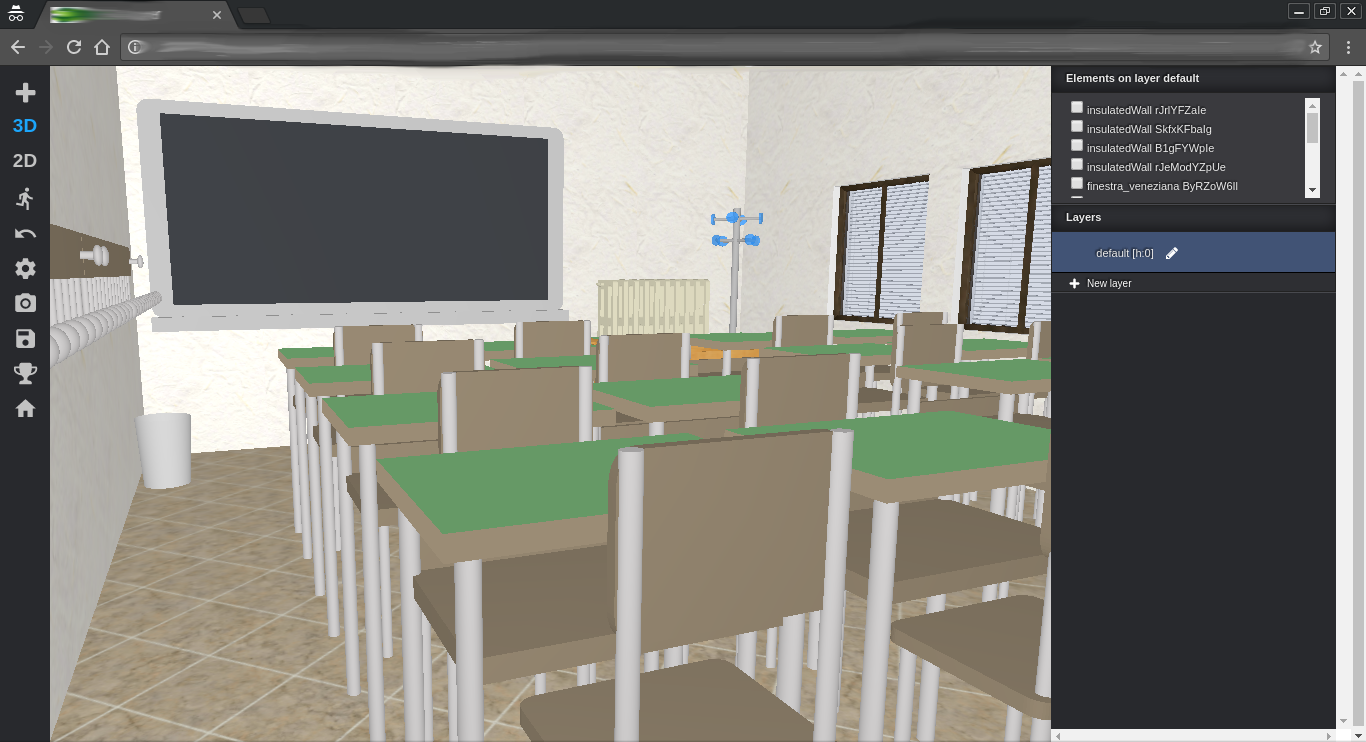
\includegraphics[width=1\linewidth]{images/3d-school}
   \caption{Schermata con visuale in prima persona}
   \label{fig:3D-school}
\end{figure}

Ogni \emph{building element} infatti comprende sia un \emph{funzione generatrice 2D (2Dgf)} e un
\emph{funzione generatrice 3D (3Dgf)}, utilizzate per ottenere modelli nella planimetria 2D e in 3D che ha generato il modello
rispettivamente.

% Once the floor-plan has been defined according to the \emph{place-and-configure} approach, the system can automatically
%  generate a 3D model which can be explored externally or in first person view, as shown in Figure~\ref{fig3D-school}.
%  Each  \emph{building element} in fact comprises either a \emph{2D generating function (2Dgf)} and a
%  \emph{3D generating function (3Dgf)}, used to obtain models used in the 2D floorplan definition and in 3D generated model
%   respectively.
